
%(BEGIN_QUESTION)
% Copyright 2015, Tony R. Kuphaldt, released under the Creative Commons Attribution License (v 1.0)
% This means you may do almost anything with this work of mine, so long as you give me proper credit

Ultrasonic, radar, and magnetostrictive level measuring instruments use the principle of {\it time-of-flight} to determine the level of a process substance in a vessel.  A critical factor for the accuracy of any time-of-flight measurement technology is the velocity of propagation for the wave in question, through the substance(s) that wave must travel.  Examine each of these illustrations and then determine which of the velocities of propagation ($v$) matter and which do not.  Be prepared to explain why, in each case!

$$\includegraphics[width=15.5cm]{i03625x01.eps}$$

$$\includegraphics[width=15.5cm]{i03625x02.eps}$$

Next, identify physical variables effecting the velocity of propagation for each of the waves in question.

\vskip 20pt \vbox{\hrule \hbox{\strut \vrule{} {\bf Suggestions for Socratic discussion} \vrule} \hrule}

\begin{itemize}
\item{} Which of these level-sensing technologies do you suspect enjoys the greatest immunity from calibration error resulting from changing process conditions?
\item{} In each case, identify factors influencing the {\it strength} of the received signal.
\end{itemize}

\underbar{file i03625}
%(END_QUESTION)





%(BEGIN_ANSWER)

\noindent
{\bf Partial answer:}

\begin{itemize}
%\item{} Ultrasonic level, top-mounted: $v_{air}$ matters, $v_{water}$ does not
\item{} Ultrasonic level, bottom-mounted: $v_{water}$ matters, $v_{air}$ does not
%\item{} Magnetostrictive level: $v_{metal}$ matters, $v_{water}$ does not, $v_{air}$ does not
%\item{} Non-contact radar level: $v_{air}$ matters, $v_{water}$ does not
\item{} GWR level: $v_{air}$ matters, $v_{water}$ does not
%\item{} GWR level/interface: $v_{air}$ and $v_{oil}$ matters, $v_{water}$ does not
\end{itemize}

The velocity of propagation for sound waves varies with the density of the medium and also its bulk modulus.  The velocity of propagation for radio waves varies with permittivity.  In both cases, changes in density (typically caused by changes in {\it pressure} and/or {\it temperature}) affect these factors, thereby affecting the velocity of propagation.
 
%(END_ANSWER)





%(BEGIN_NOTES)

{\it The questions posed here are extremely important for students to know how to answer, because they cut to the heart of how each echo-based instrument works (i.e. what factor or factors influence its ability to reliably detect level).}

\begin{itemize}
\item{} Ultrasonic level, top-mounted: $v_{air}$ matters, $v_{water}$ does not
\item{} Ultrasonic level, bottom-mounted: $v_{water}$ matters, $v_{air}$ does not
\item{} Magnetostrictive level: $v_{metal}$ matters, $v_{water}$ does not, $v_{air}$ does not
\item{} Non-contact radar level: $v_{air}$ matters, $v_{water}$ does not
\item{} GWR level: $v_{air}$ matters, $v_{water}$ does not
\item{} GWR level/interface: $v_{air}$ and $v_{oil}$ matters, $v_{water}$ does not
\end{itemize}

The velocity of sound through liquid is primarily affected by temperature.  The velocity of sound through a gas or vapor is strongly affected by temperature and pressure.

\vskip 10pt

The velocity of sound through a solid material (e.g. the rod of a magnetostrictive instrument) is weakly affected by temperature, and unaffected by pressure.

\vskip 10pt

The velocity of radio waves is weakly affected by both temperature and pressure because these factors cause the density of the medium to change, which indirectly changes the {\it electrical permittivity} of the medium.


 
%INDEX% Measurement, level: magnetostrictive
%INDEX% Measurement, level: radar
%INDEX% Measurement, level: ultrasonic

%(END_NOTES)


